\begin{figure}[H]
    \centering
    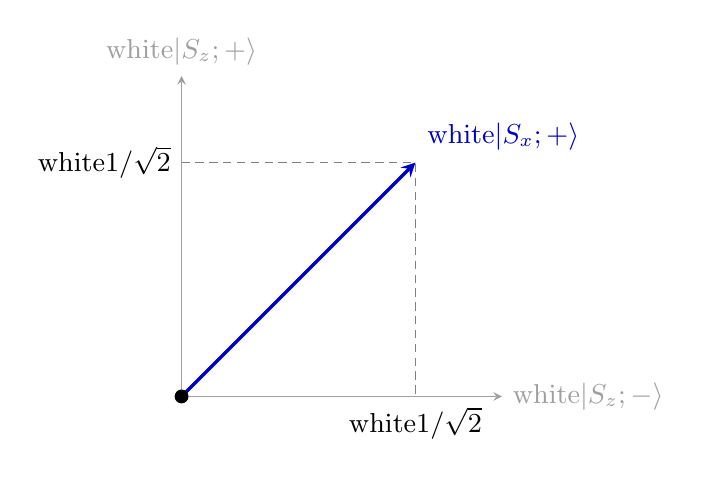
\begin{tikzpicture}[>=stealth, scale=1.1, transform shape, every node/.style={font=\small}, x={(2cm,0cm)}, y={(0cm,2cm)}]
        \coordinate (O) at (0,0);
        \coordinate (Zplus) at (0,1.35);
        \coordinate (Zminus) at (1.35,0);
        \coordinate (State) at (1.35,1.35);

        \draw[->,gray!75] (O) -- (0,1.85) node[above] {\contour{white}{$|S_z;+\rangle$}};
        \draw[->,gray!75] (O) -- (1.85,0) node[right] {\contour{white}{$|S_z;-\rangle$}};
        \draw[densely dashed,gray] (Zplus) -- (State) -- (Zminus);
        \draw[->,very thick,blue!75!black] (O) -- (State)
            node[above right] at (State) {\contour{white}{$|S_x;+\rangle$}};
        \node[left] at (Zplus) {\contour{white}{$1/\sqrt{2}$}};
        \node[below] at (Zminus) {\contour{white}{$1/\sqrt{2}$}};
        \fill (O) circle (0.04);
    \end{tikzpicture}
    \caption{Representación de las amplitudes de $|S_x;+\rangle$ en la base de $S_z$: $|S_x;+\rangle=(|S_z;+\rangle+|S_z;-\rangle)/\sqrt{2}$. Las dos amplitudes tienen módulo $1/\sqrt{2}$, por lo que cada resultado de una medición de $S_z$ tiene probabilidad $1/2$.}
    \label{fig:superposicion-spin}
\end{figure}